\begin{frame}
  
\includegraphics[width=\columnwidth]{fig/SverigesRikesLag.png}
\end{frame}

\begin{frame}
  \begin{block}{10 kap. Högskoleförordningen (1993:100)\nocite{SFS1993:100}}
    \textbf{Allmänna bestämmelser}

    \vspace{0.5em}
    1 §   Disciplinära åtgärder får vidtas mot studenter som
    \begin{enumerate}
      \item med otillåtna hjälpmedel eller på annat sätt försöker vilseleda vid 
        prov eller när en studieprestation annars ska bedömas,
      \item stör eller hindrar undervisning, prov eller annan verksamhet inom 
        ramen för utbildningen vid högskolan,
      \item stör verksamheten vid högskolans bibliotek eller annan särskild 
        inrättning inom högskolan, eller
      \item utsätter en annan student eller en arbetstagare vid högskolan för 
        sådana trakasserier eller sexuella trakasserier som avses i 1 kap. 4 § 
        diskrimineringslagen (2008:567).
    \end{enumerate}
  \end{block}
\end{frame}

\begin{frame}
  \begin{block}{10 kap. Högskoleförordningen (1993:100)\nocite{SFS1993:100}, 
    forts.}
    \textbf{Disciplinära åtgärder}

    \vspace{0.5em}
    2 § De disciplinära åtgärderna är varning och avstängning.

    \vspace{0.5em}
    Ett beslut om avstängning innebär att studenten inte får delta i 
    undervisning, prov eller annan verksamhet inom ramen för utbildningen vid 
    högskolan. Beslutet skall avse en eller flera perioder, dock sammanlagt 
    högst sex månader.

    \vspace{0.5em}
    Ett beslut om avstängning får också begränsas till att avse tillträde till 
    vissa lokaler inom högskolan.
  \end{block}
\end{frame}

\begin{frame}
  \begin{block}{10 kap. Högskoleförordningen (1993:100)\nocite{SFS1993:100}, 
    forts.}
    \textbf{Disciplinnämnden}

    \vspace{0.5em}
    3 § Ärenden om disciplinära åtgärder skall, om inte annat följer av 9 §, 
      handläggas av en disciplinnämnd. En sådan nämnd skall finnas vid varje 
      högskola.

    \vspace{0.5em}
    4 § Disciplinnämnden skall bestå av rektor som ordförande, en lagfaren 
      ledamot som skall vara eller ha varit ordinarie domare och en företrädare 
      för lärarna vid högskolan. Studenterna vid högskolan har rätt att vara 
      representerade i nämnden med två ledamöter. Förordning (1998:1003).
  \end{block}
\end{frame}

\begin{frame}
  \begin{block}{10 kap. Högskoleförordningen (1993:100)\nocite{SFS1993:100}, 
    forts.}
    13 §   När ett beslut om avstängning har fattats, skall underrättelser om 
       detta genast tillställas Centrala studiestödsnämnden och de organ inom 
       högskolan som berörs.
  \end{block}
\end{frame}

\begin{frame}
  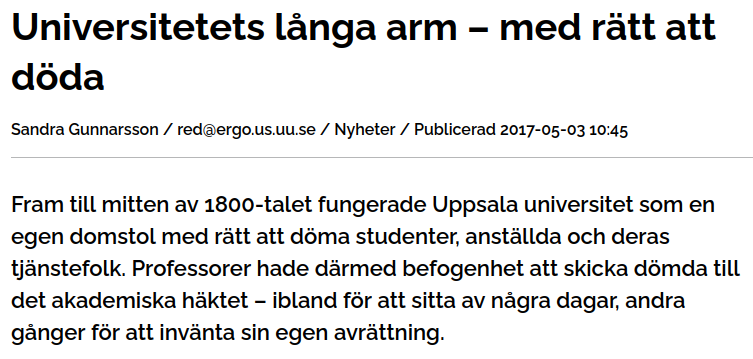
\includegraphics[width=\columnwidth]{fig/uu-domstol.png}
\end{frame}

\begin{frame}
  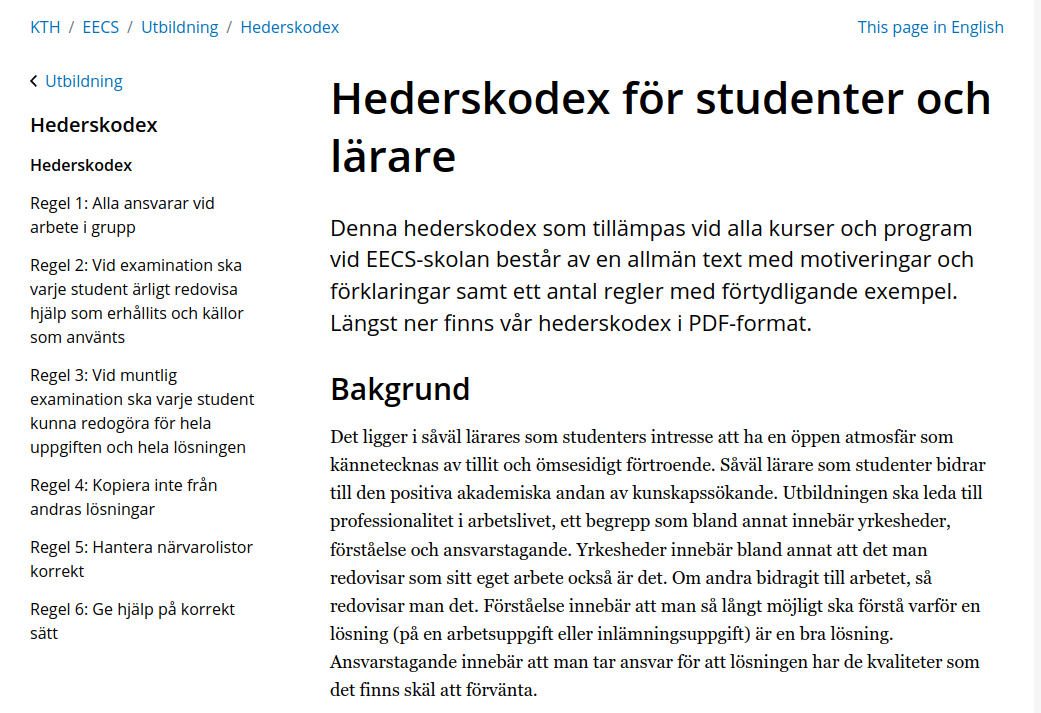
\includegraphics[width=\columnwidth]{fig/hederskodex.png}
\end{frame}
